\subsection{Stetigkeit vs Differenzierbarkeit}


\begin{Rezept}{Prüfen, ob $f$ differenzierbar an $x_0$}{}
    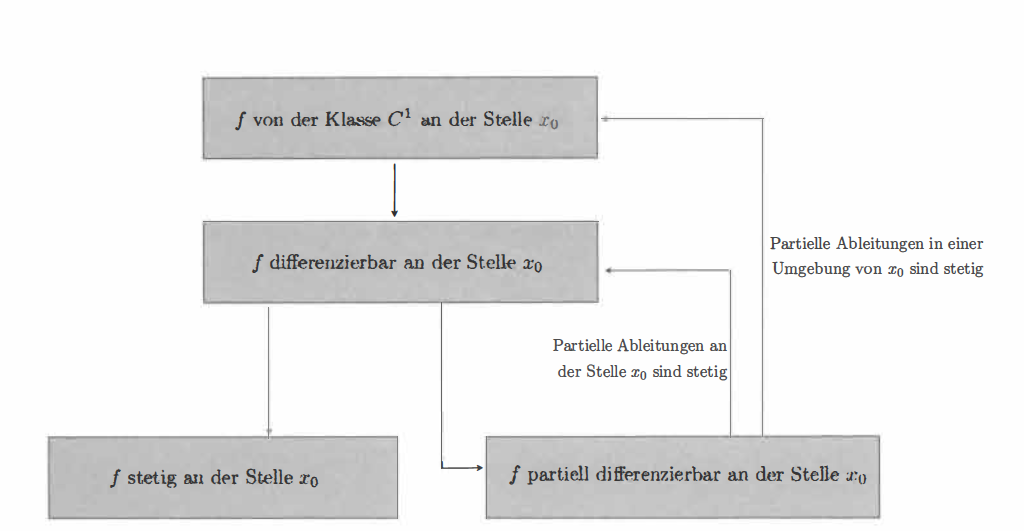
\includegraphics[width=8cm]{1}
    
    $f$ stetig an $x_0$? Nein $\Rightarrow$ $f$ nicht diffbar.\\
	$\Downarrow$ Ja\\
	Ist $f$ in $x_0$ partiell diffbar, existiert $\frac{\partial f}{\partial x_i}(x_0)$? Nein $\Rightarrow$ $f$ nicht diffbar.\\
	$\Downarrow$ Ja\\
	Ist $\frac{\partial f}{\partial x_i}(x_0)$ stetig? Ja $\Rightarrow$ $f$ ist diffbar!\\
	$\Downarrow$ Nein\\
	Existiert eine lineare Abbildung $A$: $\mathbb{R}^n \rightarrow \mathbb{R}^m$ sodass $A=\nabla f(x_0)$, also existert:
	\[
    	\lim_{x\rightarrow x_0} \frac{|f(x)-f(x_0)-\nabla f(x_0) - (x-x_0)|}{||x-x_0||}
	\]?
	Ja $\Rightarrow$ $f$ ist diffbar!\\
	Nein $\Rightarrow$ $f$ ist nicht diffbar.
\end{Rezept}
